\documentclass{article}
% Change "article" to "report" to get rid of page number on title page
\usepackage{amsmath,amsfonts,amsthm,amssymb}
\usepackage{setspace}
\usepackage{fancyhdr}
\usepackage{lastpage}
\usepackage{extramarks}
\usepackage{chngpage}
\usepackage{soul}
\usepackage[usenames,dvipsnames]{color}
\usepackage{graphicx,float,wrapfig}
\usepackage{ifthen}
\usepackage{listings}
\usepackage{courier}
\usepackage{subcaption}
\usepackage[squaren,Gray]{SIunits}
\usepackage[colorlinks,bookmarks=false,linkcolor=black,urlcolor=blue, citecolor=black]{hyperref}


%   !!!!!!!!!!!!!!!!!!!!!!!!!!!!!!!!!!!!!!!!!!!!!!!!!!!!!
%
%   Here put your info (name, due date, title etc).
%   the rest should be left unchanged.
%
%
%
%   !!!!!!!!!!!!!!!!!!!!!!!!!!!!!!!!!!!!!!!!!!!!!!!!!!!!!


% Homework Specific Information
\newcommand{\hmwkTitle}{Report 1}
\newcommand{\hmwkSubTitle}{Fourier transforms and analysis}
\newcommand{\hmwkDueDate}{12$^{\text{th}}$ Avril, 2018}
\newcommand{\hmwkClass}{Computational Physics III}
\newcommand{\hmwkClassTime}{}
%\newcommand{\hmwkClassInstructor}{Prof. Oleg Yazyev}
\newcommand{\hmwkAuthorName}{Tristan Henchoz}
%
%

% In case you need to adjust margins:
\topmargin=-0.45in      %
\evensidemargin=0in     %
\oddsidemargin=0in      %
\textwidth=6.5in        %
\textheight=9.5in       %
\headsep=0.25in         %

% This is the color used for  comments below
\definecolor{MyDarkGreen}{rgb}{0.0,0.4,0.0}

% For faster processing, load Matlab syntax for listings
\lstloadlanguages{Matlab}%
\lstset{language=Matlab,                        % Use MATLAB
        frame=single,                           % Single frame around code
        basicstyle=\small\ttfamily,             % Use small true type font
        keywordstyle=[1]\color{Blue}\bf,        % MATLAB functions bold and blue
        keywordstyle=[2]\color{Purple},         % MATLAB function arguments purple
        keywordstyle=[3]\color{Blue}\underbar,  % User functions underlined and blue
        identifierstyle=,                       % Nothing special about identifiers
                                                % Comments small dark green courier
        commentstyle=\usefont{T1}{pcr}{m}{sl}\color{MyDarkGreen}\small,
        stringstyle=\color{Purple},             % Strings are purple
        showstringspaces=false,                 % Don't put marks in string spaces
        tabsize=3,                              % 5 spaces per tab
        %
        %%% Put standard MATLAB functions not included in the default
        %%% language here
        morekeywords={xlim,ylim,var,alpha,factorial,poissrnd,normpdf,normcdf},
        %
        %%% Put MATLAB function parameters here
        morekeywords=[2]{on, off, interp},
        %
        %%% Put user defined functions here
        morekeywords=[3]{FindESS, homework_example},
        %
        morecomment=[l][\color{Blue}]{...},     % Line continuation (...) like blue comment
        numbers=left,                           % Line numbers on left
        firstnumber=1,                          % Line numbers start with line 1
        numberstyle=\tiny\color{Blue},          % Line numbers are blue
        stepnumber=1                        % Line numbers go in steps of 5
        }

% Setup the header and footer
\pagestyle{fancy}                                                       %
\lhead{\hmwkAuthorName}                                                 %
%\chead{\hmwkClass\ (\hmwkClassInstructor\ \hmwkClassTime): \hmwkTitle}  %
\rhead{\hmwkClass\ : \hmwkTitle}  %
%\rhead{\firstxmark}                                                     %
\lfoot{\lastxmark}                                                      %
\cfoot{}                                                                %
\rfoot{Page\ \thepage\ of\ \protect\pageref{LastPage}}                  %
\renewcommand\headrulewidth{0.4pt}                                      %
\renewcommand\footrulewidth{0.4pt}                                      %

% This is used to trace down (pin point) problems
% in latexing a document:
%\tracingall

%%%%%%%%%%%%%%%%%%%%%%%%%%%%%%%%%%%%%%%%%%%%%%%%%%%%%%%%%%%%%
% Some tools
\newcommand{\enterProblemHeader}[1]{\nobreak\extramarks{#1}{#1 continued on next page\ldots}\nobreak%
                                    \nobreak\extramarks{#1 (continued)}{#1 continued on next page\ldots}\nobreak}%
\newcommand{\exitProblemHeader}[1]{\nobreak\extramarks{#1 (continued)}{#1 continued on next page\ldots}\nobreak%
                                   \nobreak\extramarks{#1}{}\nobreak}%

\newlength{\labelLength}
\newcommand{\labelAnswer}[2]
  {\settowidth{\labelLength}{#1}%
   \addtolength{\labelLength}{0.25in}%
   \changetext{}{-\labelLength}{}{}{}%
   \noindent\fbox{\begin{minipage}[c]{\columnwidth}#2\end{minipage}}%
   \marginpar{\fbox{#1}}%

   % We put the blank space above in order to make sure this
   % \marginpar gets correctly placed.
   \changetext{}{+\labelLength}{}{}{}}%

\setcounter{secnumdepth}{0}
\newcommand{\homeworkProblemName}{}%
\newcounter{homeworkProblemCounter}%
\newenvironment{homeworkProblem}[1][Problem \arabic{homeworkProblemCounter}]%
  {\stepcounter{homeworkProblemCounter}%
   \renewcommand{\homeworkProblemName}{#1}%
   \section{\homeworkProblemName}%
   \enterProblemHeader{\homeworkProblemName}}%
  {\exitProblemHeader{\homeworkProblemName}}%

\newcommand{\problemAnswer}[1]
  {\noindent\fbox{\begin{minipage}[c]{\columnwidth}#1\end{minipage}}}%

\newcommand{\problemLAnswer}[1]
  {\labelAnswer{\homeworkProblemName}{#1}}

\newcommand{\homeworkSectionName}{}%
\newlength{\homeworkSectionLabelLength}{}%
\newenvironment{homeworkSection}[1]%
  {% We put this space here to make sure we're not connected to the above.
   % Otherwise the changetext can do funny things to the other margin

   \renewcommand{\homeworkSectionName}{#1}%
   \settowidth{\homeworkSectionLabelLength}{0.15in}%\homeworkSectionName}%
   \addtolength{\homeworkSectionLabelLength}{0.25in}%
   \changetext{}{-\homeworkSectionLabelLength}{}{}{}%
   \subsection{\homeworkSectionName}%
   \enterProblemHeader{\homeworkProblemName\ [\homeworkSectionName]}}%
  {\enterProblemHeader{\homeworkProblemName}%

   % We put the blank space above in order to make sure this margin
   % change doesn't happen too soon (otherwise \sectionAnswer's can
   % get ugly about their \marginpar placement.
   \changetext{}{+\homeworkSectionLabelLength}{}{}{}}%

\newcommand{\sectionAnswer}[1]
  {% We put this space here to make sure we're disconnected from the previous
   % passage

   \noindent\fbox{\begin{minipage}[c]{\columnwidth}#1\end{minipage}}%
   \enterProblemHeader{\homeworkProblemName}\exitProblemHeader{\homeworkProblemName}%
   \marginpar{\fbox{\homeworkSectionName}}%

   % We put the blank space above in order to make sure this
   % \marginpar gets correctly placed.
   }%

%%% I think \captionwidth (commented out below) can go away
%%%
%% Edits the caption width
%\newcommand{\captionwidth}[1]{%
%  \dimen0=\columnwidth   \advance\dimen0 by-#1\relax
%  \divide\dimen0 by2
%  \advance\leftskip by\dimen0
%  \advance\rightskip by\dimen0
%}

% Includes a figure
% The first parameter is the label, which is also the name of the figure
%   with or without the extension (e.g., .eps, .fig, .png, .gif, etc.)
%   IF NO EXTENSION IS GIVEN, LaTeX will look for the most appropriate one.
%   This means that if a DVI (or PS) is being produced, it will look for
%   an eps. If a PDF is being produced, it will look for nearly anything
%   else (gif, jpg, png, et cetera). Because of this, when I generate figures
%   I typically generate an eps and a png to allow me the most flexibility
%   when rendering my document.
% The second parameter is the width of the figure normalized to column width
%   (e.g. 0.5 for half a column, 0.75 for 75% of the column)
% The third parameter is the caption.
\newcommand{\scalefig}[3]{
  \begin{figure}[H]
    % Requires \usepackage{graphicx}
    \centering
    \includegraphics[width=#2\columnwidth]{#1}
    %%% I think \captionwidth (see above) can go away as long as
    %%% \centering is above
    %\captionwidth{#2\columnwidth}%
    \caption{#3}
    \label{#1}
  \end{figure}}

% Includes a MATLAB script.
% The first parameter is the label, which also is the name of the script
%   without the .m.
% The second parameter is the optional caption.
\newcommand{\matlabscript}[2]
  {\begin{itemize}\item[]\lstinputlisting[caption=#2,label=#1]{#1.m}\end{itemize}}

%%%%%%%%%%%%%%%%%%%%%%%%%%%%%%%%%%%%%%%%%%%%%%%%%%%%%%%%%%%%%


%%%%%%%%%%%%%%%%%%%%%%%%%%%%%%%%%%%%%%%%%%%%%%%%%%%%%%%%%%%%%
% Make title
%\title{\vspace{2in}\textmd{\textbf{\hmwkClass:\ \hmwkTitle\ifthenelse{\equal{\hmwkSubTitle}{}}{}{\\\hmwkSubTitle}}}\\\normalsize\vspace{0.1in}\small{Due\ on\ \hmwkDueDate}\\\vspace{0.1in}\large{\textit{\hmwkClassInstructor\ \hmwkClassTime}}\vspace{3in}}
\title{\vspace{2in}\textmd{\textbf{\hmwkClass:\ \hmwkTitle\ifthenelse{\equal{\hmwkSubTitle}{}}{}{\\\hmwkSubTitle}}}\\\normalsize\vspace{0.1in}\small{Due\ on\ \hmwkDueDate}\\\vspace{0.1in}\large{\textit{ \hmwkClassTime}}\vspace{3in}}
\date{}
\author{\textbf{\hmwkAuthorName}}
%%%%%%%%%%%%%%%%%%%%%%%%%%%%%%%%%%%%%%%%%%%%%%%%%%%%%%%%%%%%%

\begin{document}
\begin{spacing}{1.1}
\maketitle
% Uncomment the \tableofcontents and \newpage lines to get a Contents page
% Uncomment the \setcounter line as well if you do NOT want subsections
%       listed in Contents
%\setcounter{tocdepth}{1}
\newpage
\tableofcontents
\newpage

% When problems are long, it may be desirable to put a \newpage or a
% \clearpage before each homeworkProblem environment

\newpage

\section*{Introduction}

To analyse many subject, it is useful to be in the reciprocal space. The Fourier transform allows a transformation from the real space to this reciprocal. For programming, it's better to operates with discretised data, which is possible with the discrete Fourier transform(DFT). The fast Fourier transform (FFT) is also a discrete Fourier transform, giving the exact same result, but in a more efficient way.

\newpage

\begin{homeworkProblem}


This part consists of coding an implementation of the DFT's algorithm, and then it is used to analyse a HCl's interferograms' data.

    \begin{homeworkSection}{(1) Implementation of DFT}
    The first part consisted of implementing the DFT's algorithm. The discrete Fourier transform $\hat{f}_{m_{m \in \mathbb{N}}}$ from a $f_{n_{n \in \mathbb{N}}}$ array of size $N$ as given in the lecture note is
        \begin{equation}
            \hat{f}_m = \sum\limits_{n=0}^{N-1} f_n e^{- 2 \pi i \cdot m \cdot n / N}
        \end{equation}
        
    \matlabscript{MatLab/mydft}{A script which does the discrete Fourier transform.}
    \end{homeworkSection}

    \begin{homeworkSection}{(2) HCl interferogram}
        The aim of the present exercise is to study the absorption spectrum of a simple linear biatomic molecule formed by one hydrogen atom (M$_{\text{H}}$ = 1.0078 a.m.u.) and one Chlorine atom. The Chlorine atom has two stable isotope $^{35}$Cl (75.77\% M$_{^{35}\text{Cl}}$ = 34.969 a.m.u.) and $^{37}$Cl (24.23\% M$_{^{37}\text{Cl}}$ = 36.966 a.m.u.). In typical IR spectroscopy experiments the collected data are interferograms, that is, records of the intensity of the light coming out of an interferometer as a function of the optical path variation induced by a movable mirror. Since the IR sources employed in the experiments contain components in a broad range of frequencies (typically [1000 - 8000] cm$^{-1}$), the interference figures result from a superposition of all these frequencies.
    \end{homeworkSection}

    \begin{homeworkSection}{(2.1) Plotting data}
        The figure~\ref{HCL_fig1} show the results obtained by the interferometer with and without sample. The central maxima is caused by a constructive interference, since the distance travelled by both light is the same.
        \begin{figure}[H]
            \begin{subfigure}{0.48\linewidth}
                \centering
                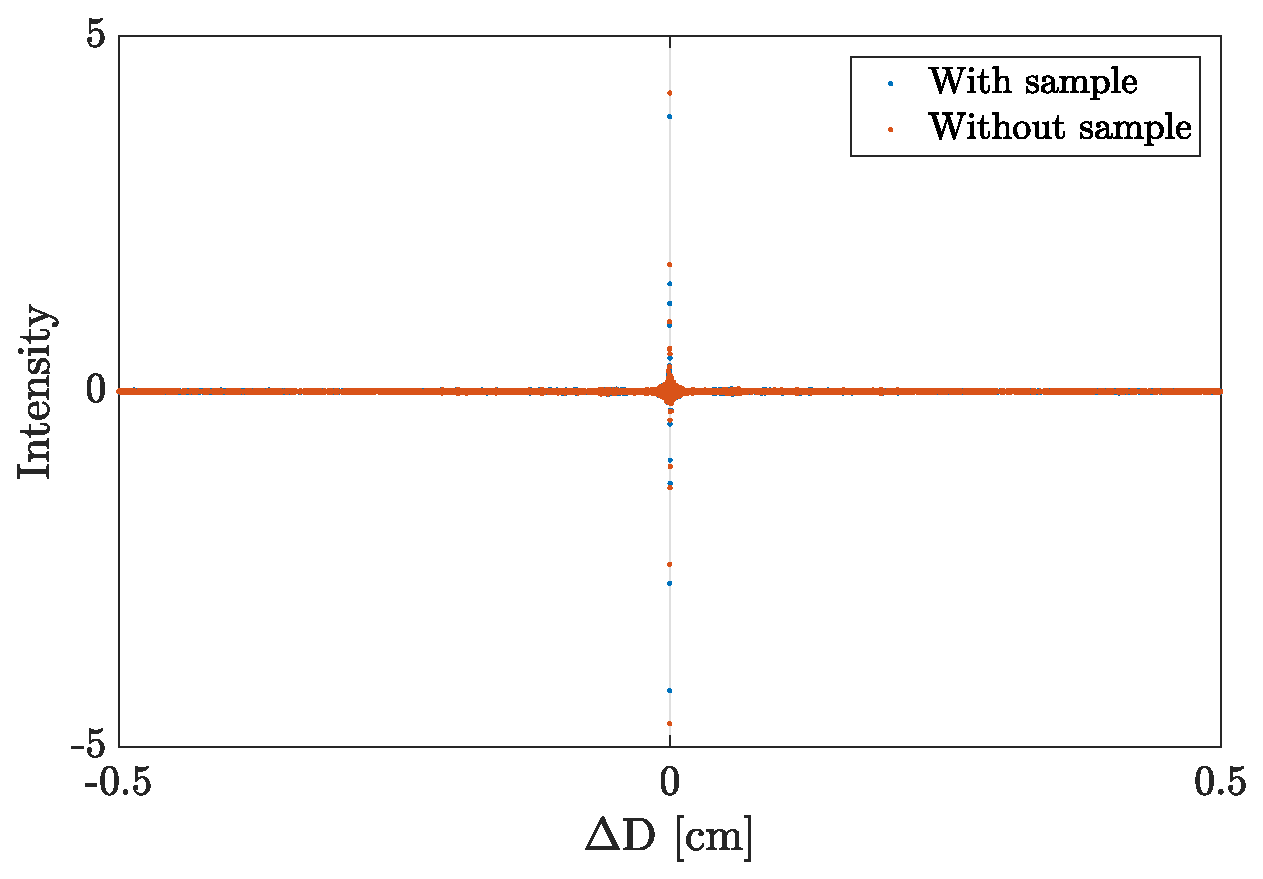
\includegraphics[height=4.9cm]{figs/HCL_fig1}
                \subcaption{Full result of the interferometer}
            \end{subfigure}
            \begin{subfigure}{0.48\linewidth}
                \centering
                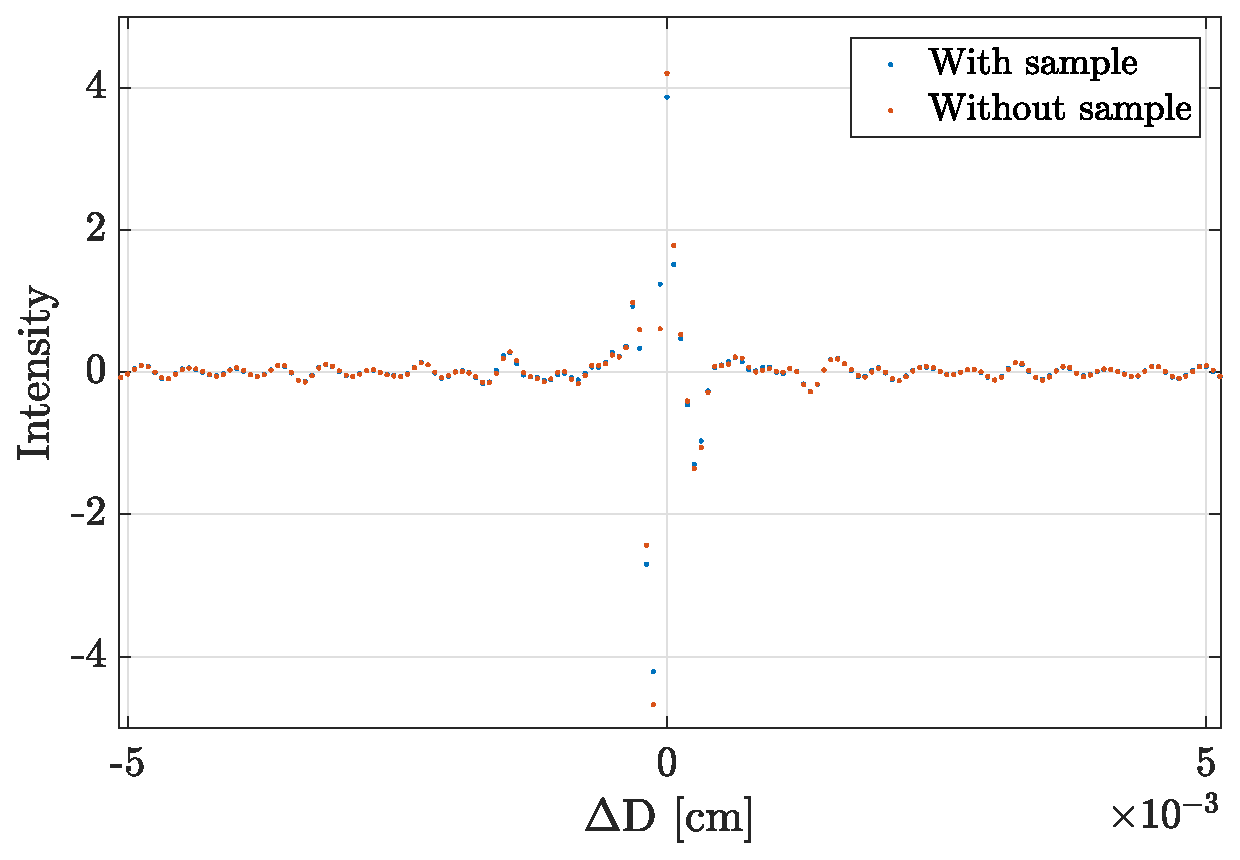
\includegraphics[height=4.8cm]{figs/HCL_fig1_1}
                \subcaption{Zoom on the central maxima}
            \end{subfigure}
            \caption{Result of the interferometer with the central maxima}
            \label{HCL_fig1}
        \end{figure}
    \end{homeworkSection}

    \begin{homeworkSection}{(2.2) Fourier transform}
        \begin{figure}[H]
            \begin{subfigure}{0.48\linewidth}
                \centering
                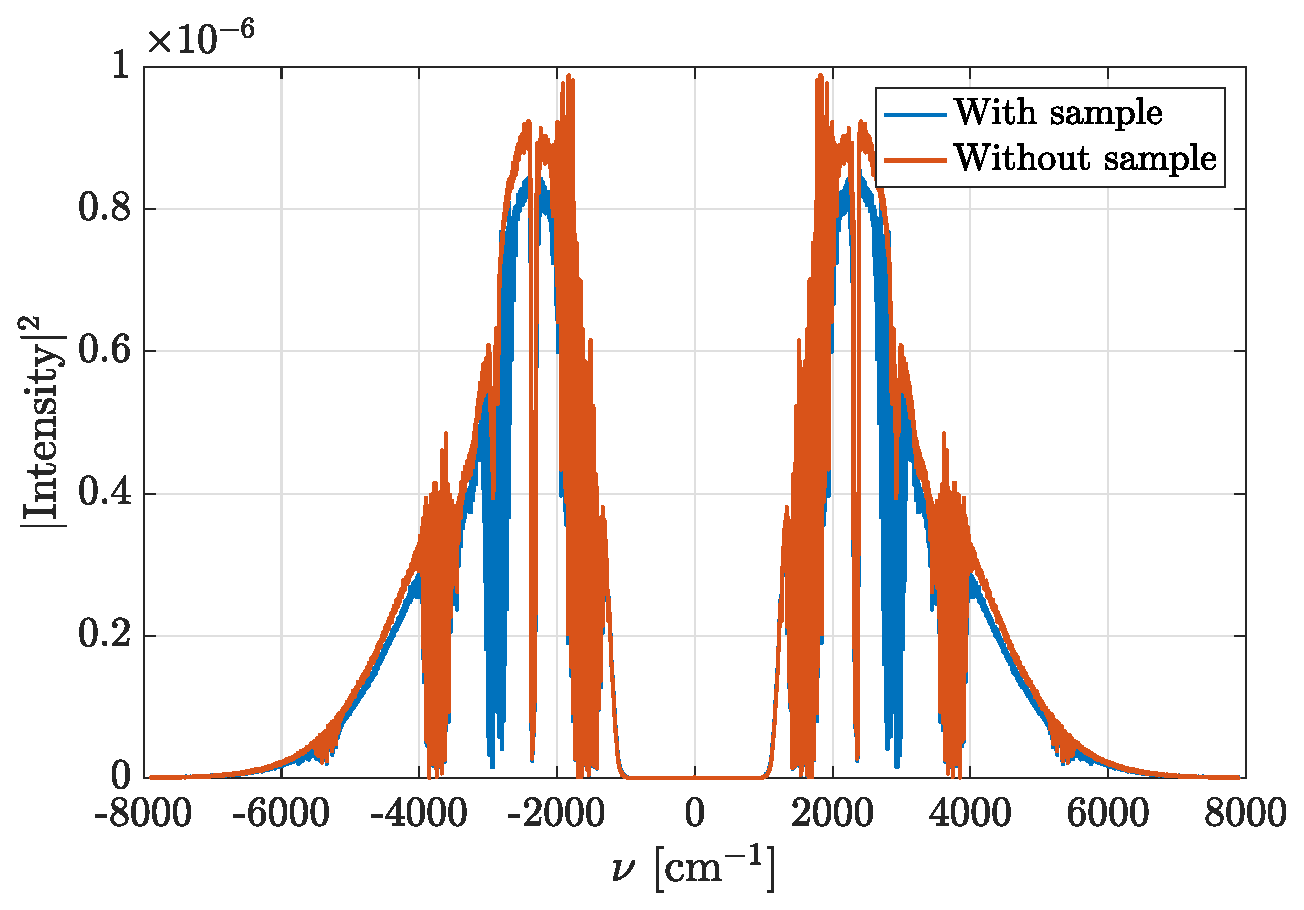
\includegraphics[height=4.9cm]{figs/HCL_fig2}
                \subcaption{Full frequency}
            \end{subfigure}
            \begin{subfigure}{0.48\linewidth}
                \centering
                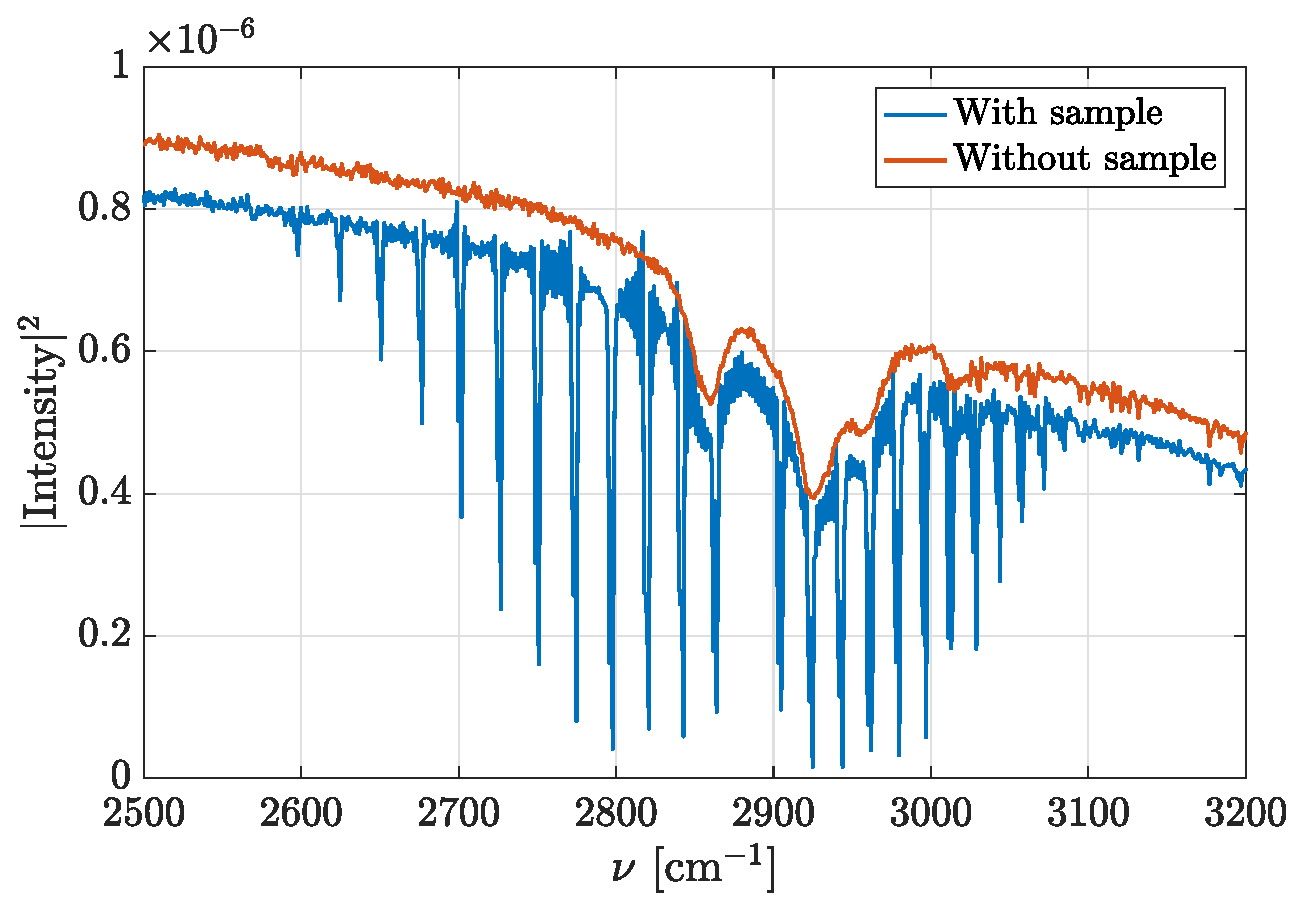
\includegraphics[height=4.9cm]{figs/HCL_fig2_2}
                \subcaption{Zoom on 2500 to 3200 cm$^{-1}$}
            \end{subfigure}
            \caption{Square modulus of the intensity of both spectra in Fourier space}
            \label{HCL_fig2}
        \end{figure}
    \end{homeworkSection}

    \begin{homeworkSection}{(2.3) Absorption spectrum}
        \scalefig{figs/HCL_fig3}{0.79}{Absorption spectrum between 2500 to 3200 cm$^{-1}$}
    \end{homeworkSection}
    
    \newpage

    \begin{homeworkSection}{(2.4) Transitions $J = 0 \leftarrow 1$ and $J = 1 \leftarrow 0$}
        As it can be seen on figure~\ref{figs/HCL_fig4}, the peaks corresponding to the transitions $J = 0 \leftarrow 1$ and $J = 1 \leftarrow 0$ are a convolution of two peaks. Calculating the area below the two peaks and subtracting the noise give us the information that the small one correspond to 31.41\% and 33.46\% of the total area of the first, respectively the second peaks. Given the fact that the Chlorine atom has two stable isotope, and is composed as 24.23\% of $^{37}$Cl, it is appropriate to think that the two smaller peaks correspond to the $^{37}$Cl and the two bigger ones to the $^{35}$Cl isotope.
        \scalefig{figs/HCL_fig4}{0.8}{Zoom on the absorption spectrum between 2858 to 2912 cm$^{-1}$}
    \end{homeworkSection}

    \begin{homeworkSection}{(2.5) Bond length of HCl}
        The frequency separation between two rotational excitation corresponding to $J = 0 \leftarrow \bar{J}$ and $J = \bar{J} \leftarrow 0$ (valid for low $\bar{J}$) is given by
        \begin{equation}
            \Delta \nu = \frac{\hbar \bar{J}(\bar{J} + 1)}{2 \pi c \mu d^2}, \mu = \frac{M_\text{H}M_\text{Cl}}{M_\text{H}+M_\text{Cl}}
        \end{equation}
        where $\mu$ is the reduced mass, $d$ the bond length and $c$ the speed of light. Converting this formula and using 41~\reciprocal{\centi\meter}~for $\Delta \nu$, as show in figure~\ref{figs/HCL_fig4}, the bond length of HCl obtained is 1.2957~\angstrom~for $^{35}$Cl and 1.2948~\angstrom~for $^{37}$Cl.
    \end{homeworkSection}

\end{homeworkProblem}

\newpage

\begin{homeworkProblem}


This part consists of coding an implementation of a FFT's algorithm, and then use it to analyse a picture of graphene.

    \begin{homeworkSection}{(1) Implementation of FFT}
    The first part consisted of implementing the radix-2 algorithm. This algorithm works with array of size $N = 2^m$ only. It is given by the following formula
        \begin{equation}
            \hat{f}[k] = \hat{e}[k] + W^k_N \hat{o}[k],\,\, W^k_N = e^{-\frac{2\pi i}{N}k}
        \end{equation}
        where $\hat{e}$ and $\hat{o}$ are the Fourier transform of the the even indices, respectively the odd indices.
        
    \matlabscript{MatLab/myfft}{A script which does the fast Fourier transform.}
    \end{homeworkSection}
    
\newpage

    \begin{homeworkSection}{(2) Bilayer graphene}
        Graphene is a well-known two-dimensional material consisting of a honeycomb lattice of carbon atoms. When two layers of graphene are placed on top of each other (bilayer graphene), the orientation of the respective lattices can differ. The mutual orientation of the lattices in the two layers is described by twist angle $\Theta$. % (see figure~\ref{Graphene_fig1})
        
        \scalefig{figs/Graphene_fig1}{0.45}{Transmission electron microscopy image of a bilayer graphene sample.}
        
        Figure~\ref{figs/Graphene_fig1} shows a transmission electron microscopy (TEM) image of bilayer graphene with two regions on the left and right of the image characterised by different twist angles, forming distinct Moiré patterns. On the top-left of the picture, a small part shows a single layer of graphene. The goal of this exercise is to use 2D Fourier transforms to analyse this data and to find the mutual orientation of the two layers in the left and in the right part of the image.
    \end{homeworkSection}

    \begin{homeworkSection}{(2.1) Conversion to grayscale}
        \scalefig{figs/Graphene_fig2}{0.45}{Conversion to grayscale image}
    \end{homeworkSection}

\newpage

    \begin{homeworkSection}{(2.2) Fourier transform}
        %\scalefig{Graphene_fig3}{0.6}{Hello}
        \scalefig{figs/Graphene_fig3_1}{0.45}{Figure~\ref{figs/Graphene_fig2} after Fourier transform; a linear transformation was apply to see clearly the Bragg peaks}
    \end{homeworkSection}

    \begin{homeworkSection}{(2.3) Peaks in Fourier space}
        The Fourier transform highlights the frequency on given direction. For honeycomb lattice as in graphene, this involves 6 peaks, two for each direction. In figure~\ref{figs/Graphene_fig3_1}, the central peak is there because everything has a zero frequency, and there are 6 groups of 3 peaks because there are three layer of graphene.
    \end{homeworkSection}

    \begin{homeworkSection}{(2.4) Fourier filter}
    \label{test}
        \begin{figure}[H]
            \begin{subfigure}{0.45\linewidth}
                \centering
                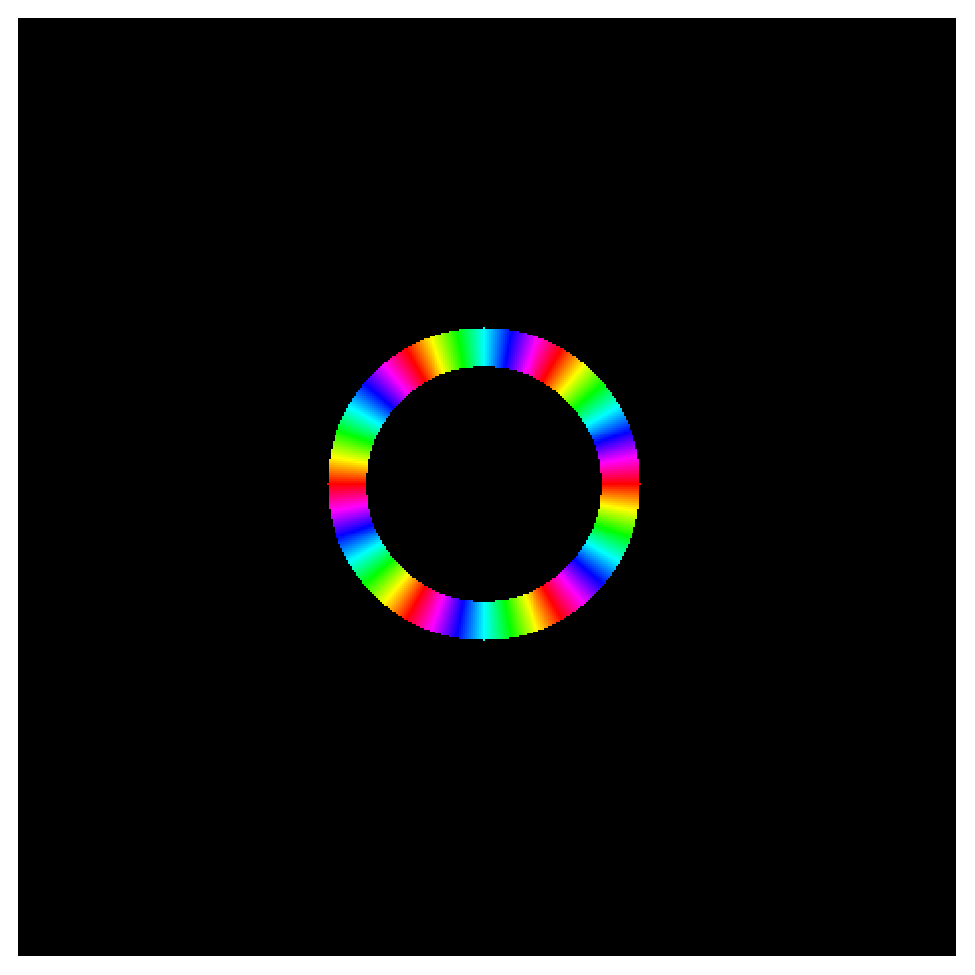
\includegraphics[height=5.5cm]{figs/Graphene_fig4}
                \subcaption{Ring filter used}
            \end{subfigure}
            \begin{subfigure}{0.52\linewidth}
                \centering
                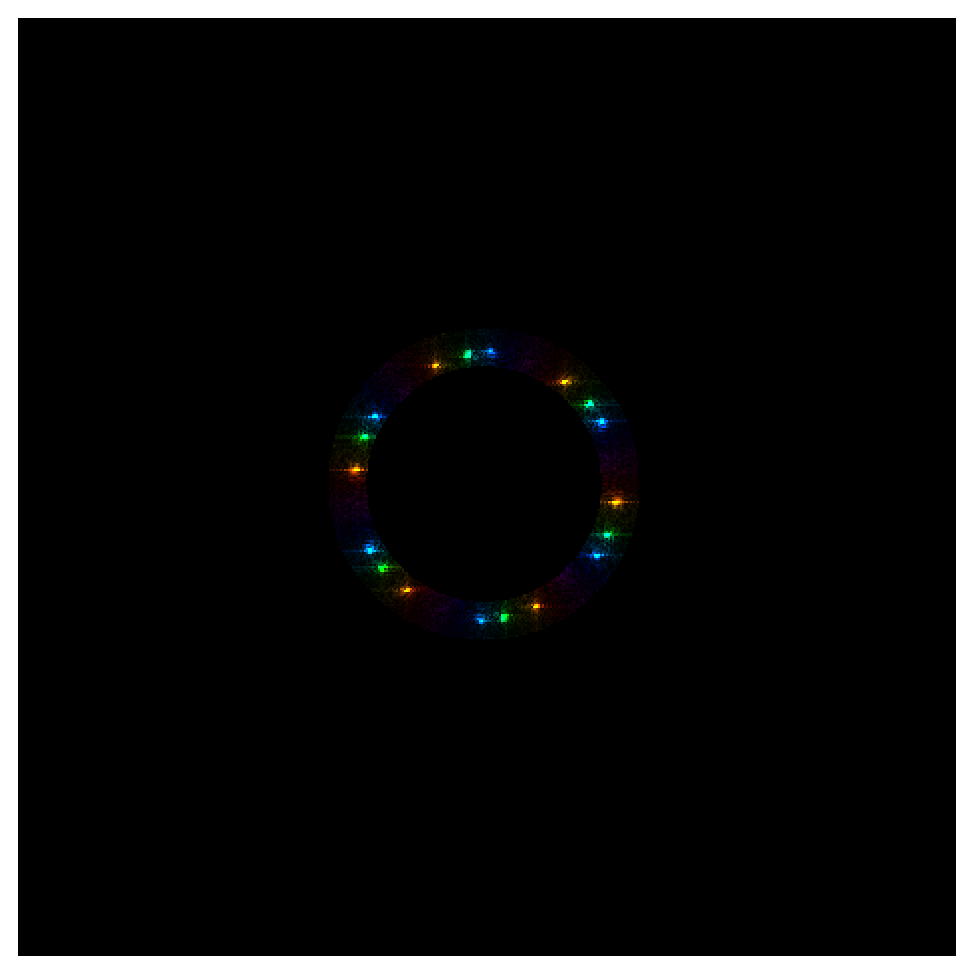
\includegraphics[height=5.5cm]{figs/Graphene_fig5_1}
                \subcaption{Fourier transform after the application of the filter}
                \label{Graphene_fig5}
            \end{subfigure}
            \caption{Fourier filter and application to distinguish the domains with different orientations.}
            \label{Graphene_fig4-5}
        \end{figure}
        %\scalefig{Graphene_fig5}{0.6}{Hello}
        %\scalefig{Graphene_fig5_2}{0.6}{Hello}
    \end{homeworkSection}

    \begin{homeworkSection}{(2.5) Inverse Fourier transform}
        Before doing the inverse Fourier transform, the figure~\ref{Graphene_fig5} was decomposed in three grayscale image, one for each colour (RGB). The inverse Fourier transform then give the three picture in figure~\ref{Graphene_fig6-8}, which combined together produce the figure~\ref{figs/Graphene_fig9}.
        \begin{figure}[H]
            \begin{subfigure}{0.33\linewidth}
                \centering
                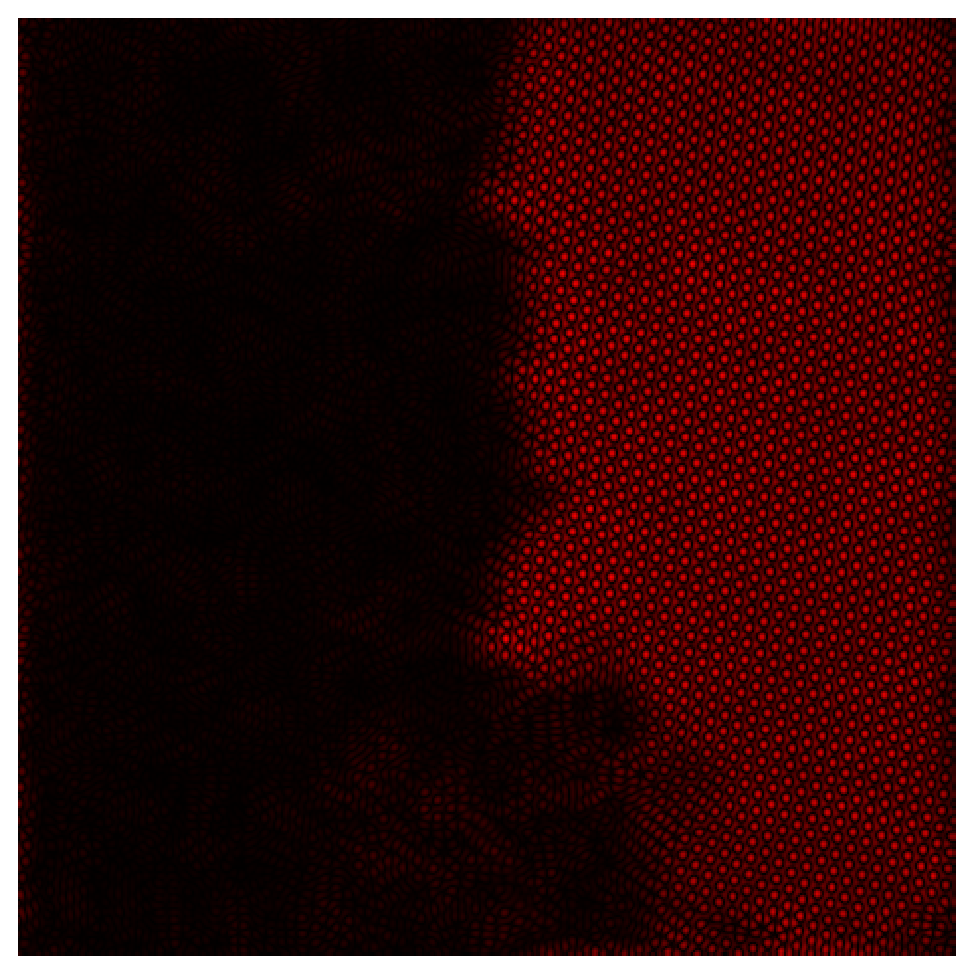
\includegraphics[height=4.5cm]{figs/Graphene_fig6}
                \subcaption{Red Filter}
            \end{subfigure}
            \begin{subfigure}{0.33\linewidth}
                \centering
                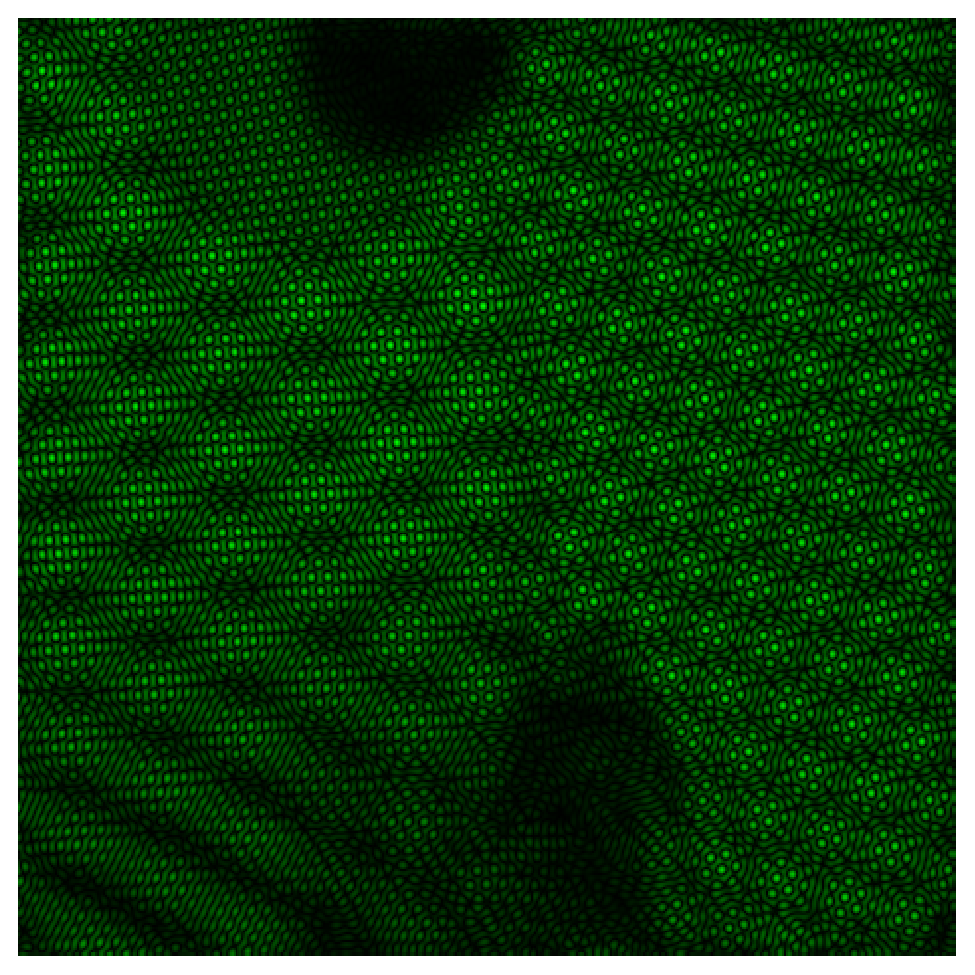
\includegraphics[height=4.5cm]{figs/Graphene_fig7}
                \subcaption{Green Filter}
            \end{subfigure}
            \begin{subfigure}{0.33\linewidth}
                \centering
                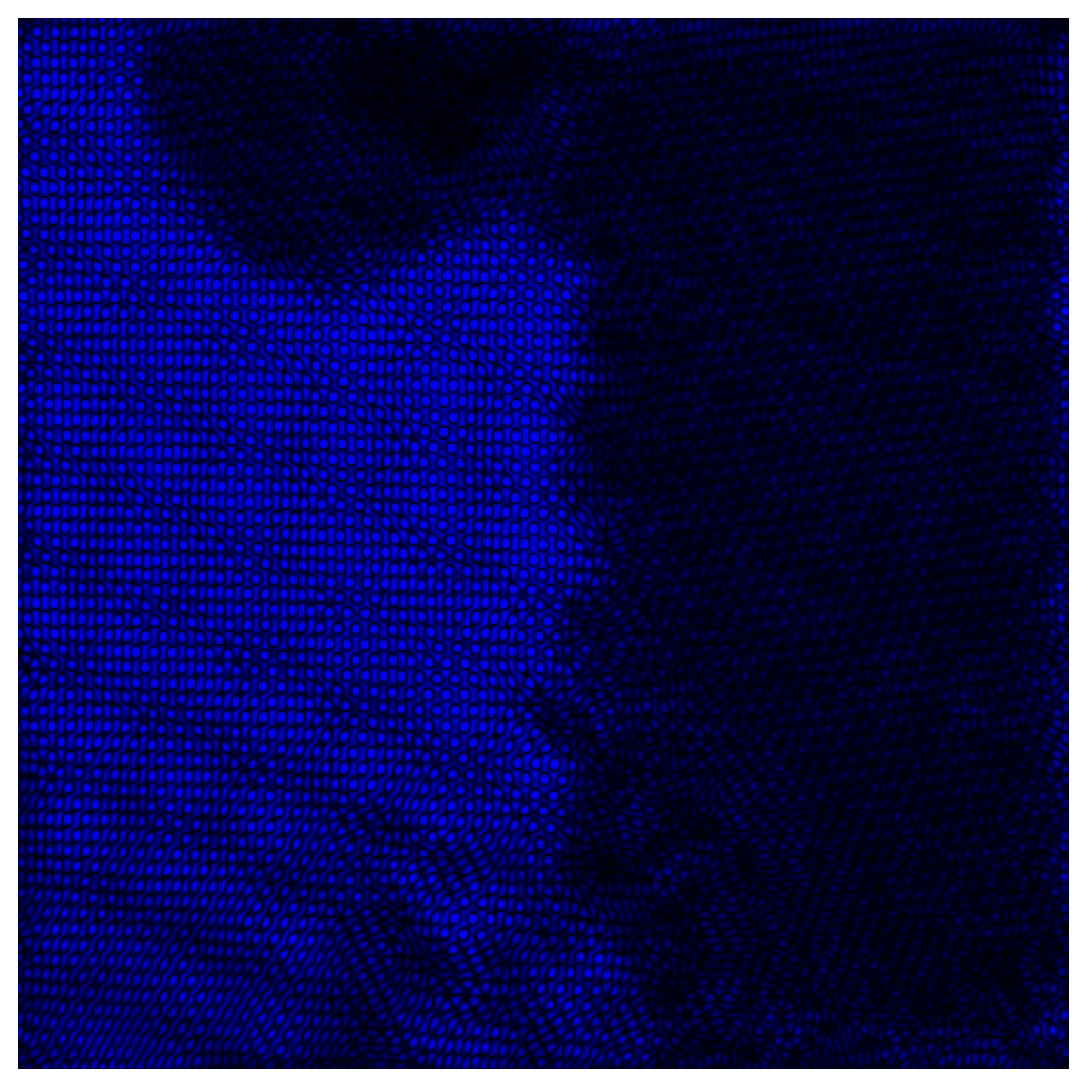
\includegraphics[height=4.5cm]{figs/Graphene_fig8}
                \subcaption{Blue Filter}
            \end{subfigure}
            \caption{Fourier inverse apply to each layer, separately.}
            \label{Graphene_fig6-8}
        \end{figure}
        
        One can see in figure~\ref{Graphene_fig6-8} that each colour corresponds to one layer of graphene; Red for the right, Blue on the left and Green on the background.
        
        \scalefig{figs/Graphene_fig9}{0.6}{Result obtained after combining the three layer}
        
        The figure~\ref{figs/Graphene_fig9} is not as clear as the one in the instruction notes. This could be explained because of the filter used, which is a continued one instead of discrete one. An other explanation is how the figure~\ref{Graphene_fig5} is made. As the figure~\ref{figs/Graphene_fig3_1} isn't totally black or white, this figure is not totally black or in color.
    \end{homeworkSection}

    \begin{homeworkSection}{(2.6) Lattice constant}
        As seen in the section above, the peaks in the Fourier space correspond to the frequency. The relation between that and the lattice constant $\lambda$~[\angstrom] :
        \begin{equation}
            \lambda = \frac{\Delta x N}{R_{px}}
        \end{equation}
        where $\Delta x = 0.3$~\angstrom~the conversion from pixel (px) to \angstrom, $N = 474$px the size of the image in pixel and $R_{px}$ the radius in pixel in the Fourier space.
        
        To obtain the radius, some hypothesis were made. The first one is that the figure~\ref{Graphene_fig5} represent a circle centre in the image. A second one was that for each peaks on this picture, the brightest pixel is the centre of the peaks. With this hypothesis, the matlab's script find the brightest pixel for each colour in the figure~\ref{Graphene_fig5} and calculate the average distance to the centre of the image for this three points only. The lattice constant obtained with this method was 2.1475~\angstrom.
        
        This could be improved by taking all the 18 peaks in Fourier space to calculate the radius, and by taking the centre of the peak, which are not always the brightest.
    \end{homeworkSection}

    \begin{homeworkSection}{(2.7) Misorientation angles}
        For this part, the same hypothesis as the point~(2.6) were made. As the peaks in Fourier space correspond to the repetition of the honeycomb's lines, there orientation correspond to the layer of graphene's orientation. The orientations of the three colour were made by finding the brightest pixel for each colour, and perform an arctan to find the $\phi$ coordinate of the peaks in polar coordinates, modulo 60$^\circ$ because an hexagon is the same with this angle. Then, the difference of orientation between the blue and green filter, respectively the red and green, were calculate to obtain the misorientation on the left$\Theta_{\text{left}}$, respectively on the right $\Theta_{\text{right}}$, of the image. The results were $\Theta_{\text{left}} = 10.47^\circ$ and $\Theta_{\text{right}} = 14.04^\circ$.
        
        This could also be improved the same way it is possible in point~(2.6).
    \end{homeworkSection}

\end{homeworkProblem}

\newpage

%			Bibliographie
\begin{thebibliography}{99}

\bibitem{notice_gen}

\textit{Exercise sessions 2–3: Discrete Fourier transform. FT-IR spectroscopy of HCl molecule.} written by O. Yazyev, D. Pasquier, M. Pizzochero, R. Fournier in 2017-2018

\bibitem{laBible}

\textit{Exercise sessions 4-5: Fast Fourier transform. Image filtering.} written by O. Yazyev, D. Pasquier, M. Pizzochero, R. Fournier in 2017-2018

\bibitem{ref}

"Technical data for Carbon", \url{http://www.periodictable.com/Elements/006/data.html}, consulted the 11$^{\text{th}}$ mars 2018

\end{thebibliography}

\end{spacing}
\end{document}

%%%%%%%%%%%%%%%%%%%%%%%%%%%%%%%%%%%%%%%%%%%%%%%%%%%%%%%%%%%%%

